\section{Detailed Step-by-Step Execution}
\label{section_appendix_step_by_step}

This section provides a detailed step-by-step exploration of the graph shown in Figure \ref{fig_imperfect_maze_exploration}. The process is illustrated for all three agents, with each step specifying the intervals calculated for each child node. Nodes that would create cycles are marked in red, and the corresponding edges are represented as dotted lines. To maintain clarity and conciseness, some straightforward steps, such as those involving simple backtracking or non-decision points, are omitted. This ensures a focused understanding of how the agents navigate and construct their respective exploration trees.

The following figures present the step-by-step exploration process for each agent, highlighting their decisions and progress throughout the graph.

\begin{figure}[H]
    \centering
    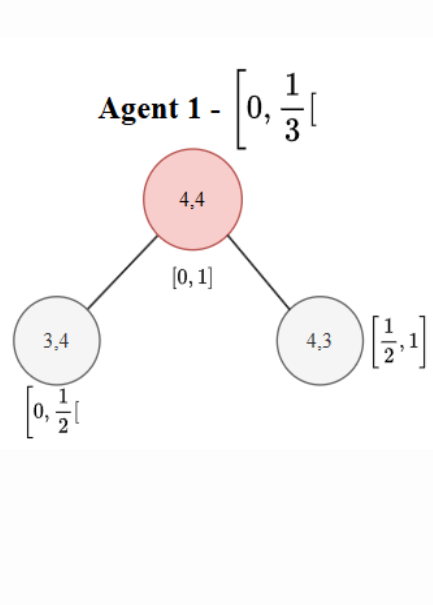
\includegraphics[width=0.8\textwidth]{ApeA/maze_agent_1_step_0.png}
    \caption{Agent 1 - Starting Node for graph from Figure \ref{fig_imperfect_maze_exploration}.}
    \label{fig_agent_1_step_0}
\end{figure}

\begin{figure}[H]
    \centering
    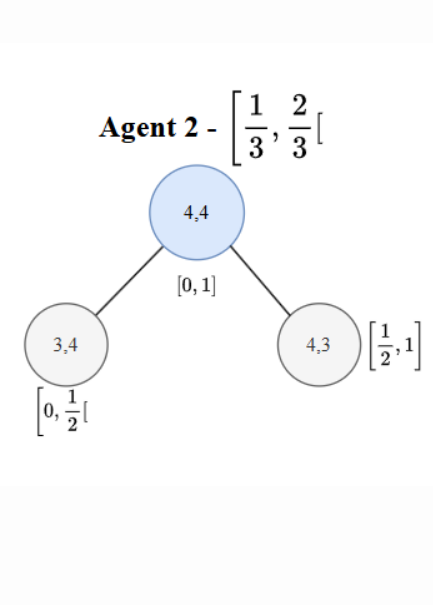
\includegraphics[width=0.8\textwidth]{ApeA/maze_agent_2_step_0.png}
    \caption{Agent 2 - Starting Node for graph from Figure \ref{fig_imperfect_maze_exploration}.}
    \label{fig_agent_2_step_0}
\end{figure}

\begin{figure}[H]
    \centering
    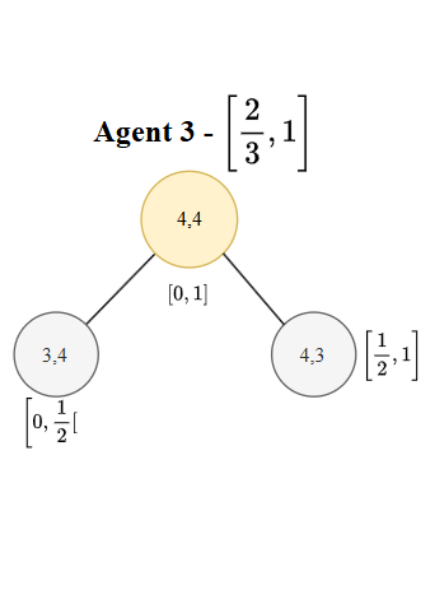
\includegraphics[width=0.8\textwidth]{ApeA/maze_agent_3_step_0.png}
    \caption{Agent 3 - Starting Node for graph from Figure \ref{fig_imperfect_maze_exploration}.}
    \label{fig_agent_3_step_0}
\end{figure}

\begin{figure}[H]
    \centering
    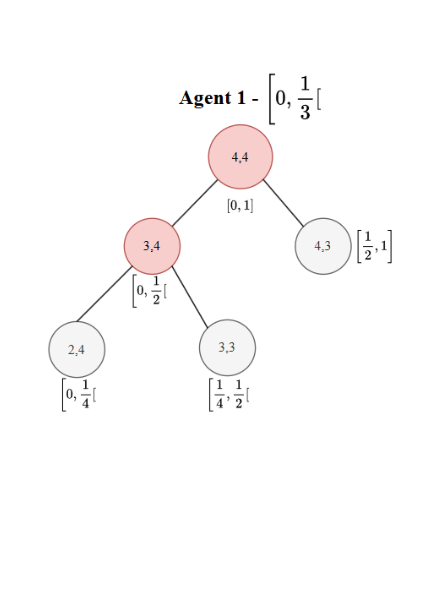
\includegraphics[width=0.8\textwidth]{ApeA/maze_agent_1_step_1.png}
    \caption{Agent 1 - First Step exploring the graph.}
    \label{fig_agent_1_step_1}
\end{figure}

\begin{figure}[H]
    \centering
    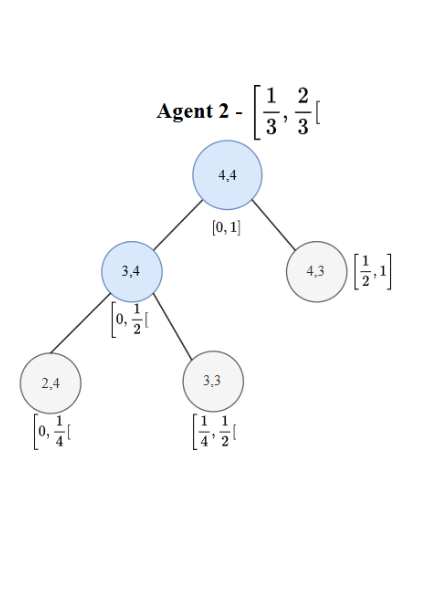
\includegraphics[width=0.8\textwidth]{ApeA/maze_agent_2_step_1.png}
    \caption{Agent 2 - First Step exploring the graph.}
    \label{fig_agent_2_step_1}
\end{figure}

\begin{figure}[H]
    \centering
    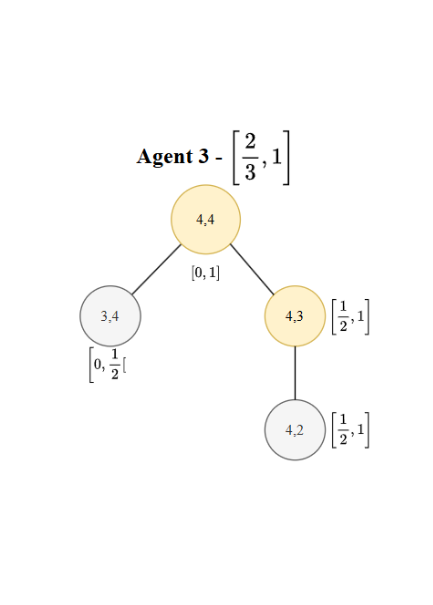
\includegraphics[width=0.8\textwidth]{ApeA/maze_agent_3_step_1.png}
    \caption{Agent 3 - First Step exploring the graph.}
    \label{fig_agent_3_step_1}
\end{figure}

\begin{figure}[H]
    \centering
    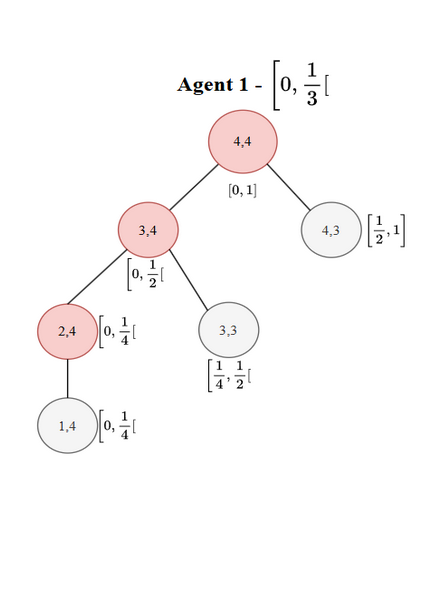
\includegraphics[width=0.8\textwidth]{ApeA/maze_agent_1_step_2.png}
    \caption{Agent 1 - Second Step exploring the graph.}
    \label{fig_agent_1_step_2}
\end{figure}

\begin{figure}[H]
    \centering
    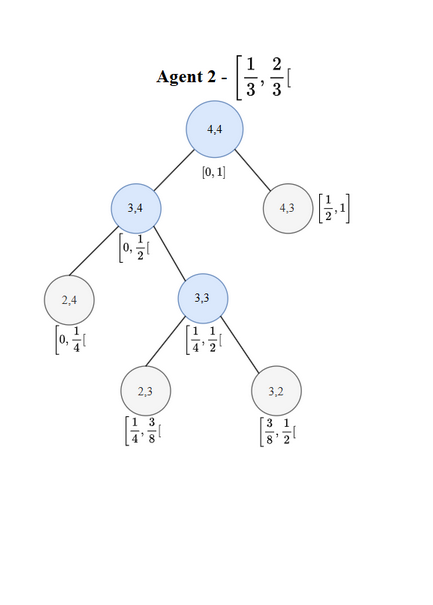
\includegraphics[width=0.8\textwidth]{ApeA/maze_agent_2_step_2.png}
    \caption{Agent 2 - Second Step exploring the graph.}
    \label{fig_agent_2_step_2}
\end{figure}

\begin{figure}[H]
    \centering
    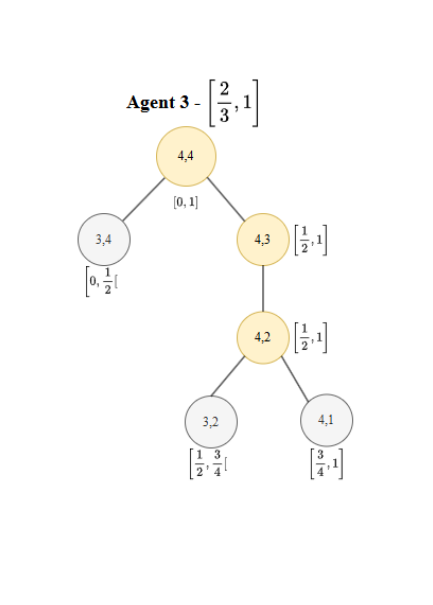
\includegraphics[width=0.8\textwidth]{ApeA/maze_agent_3_step_2.png}
    \caption{Agent 3 - Second Step exploring the graph.}
    \label{fig_agent_3_step_2}
\end{figure}

\begin{figure}[H]
    \centering
    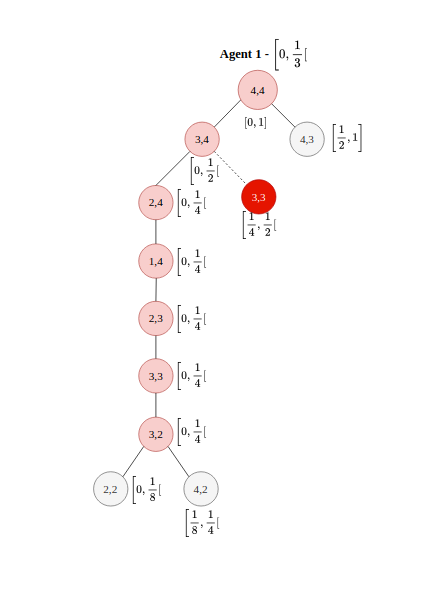
\includegraphics[width=0.8\textwidth]{ApeA/maze_agent_1_step_3.png}
    \caption{Agent 1 - Multiple Steps of exploration.}
    \label{fig_agent_1_step_3}
\end{figure}

\begin{figure}[H]
    \centering
    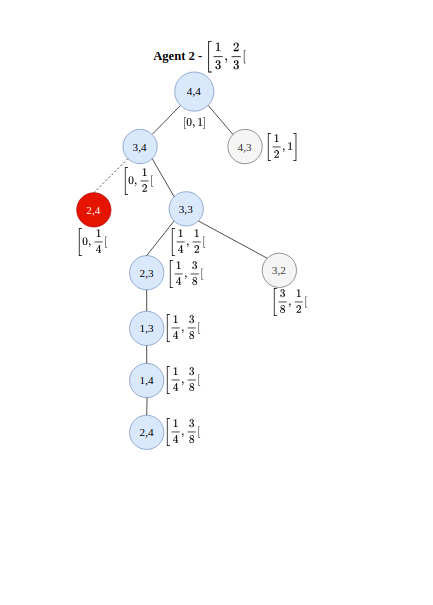
\includegraphics[width=0.8\textwidth]{ApeA/maze_agent_2_step_3.png}
    \caption{Agent 2 - Multiple Steps of exploration.}
    \label{fig_agent_2_step_3}
\end{figure}

\begin{figure}[H]
    \centering
    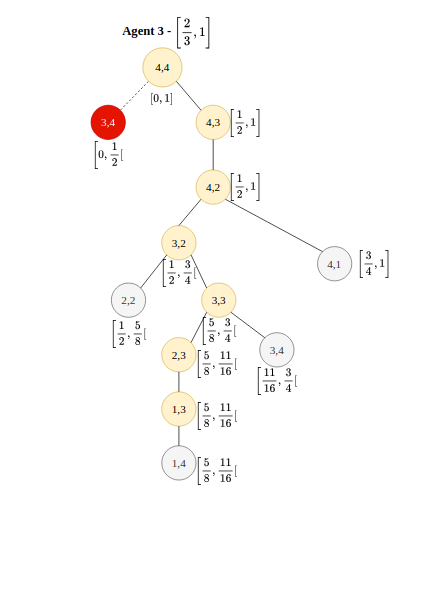
\includegraphics[width=0.8\textwidth]{ApeA/maze_agent_3_step_3.png}
    \caption{Agent 3 - Multiple Steps of exploration.}
    \label{fig_agent_3_step_3}
\end{figure}

\begin{figure}[H]
    \centering
    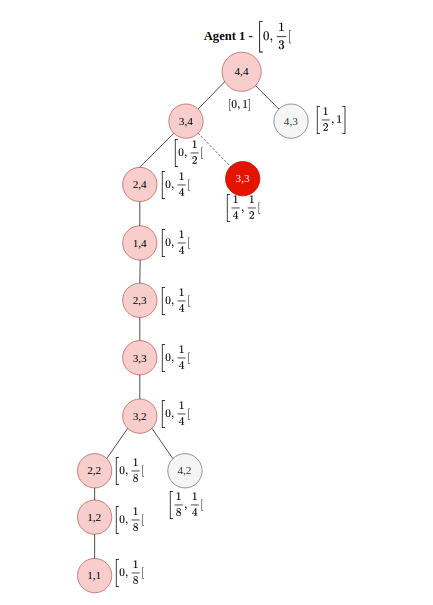
\includegraphics[width=1\textwidth]{ApeA/maze_agent_1_step_4.png}
    \caption{Agent 1 - Final exploration steps.}
    \label{fig_agent_1_step_4}
\end{figure}

\begin{figure}[H]
    \centering
    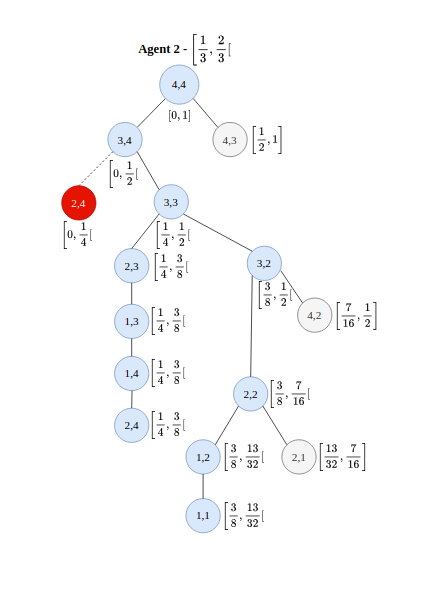
\includegraphics[width=1\textwidth]{ApeA/maze_agent_2_step_4.png}
    \caption{Agent 2 - Final exploration steps.}
    \label{fig_agent_2_step_4}
\end{figure}

\begin{figure}[H]
    \centering
    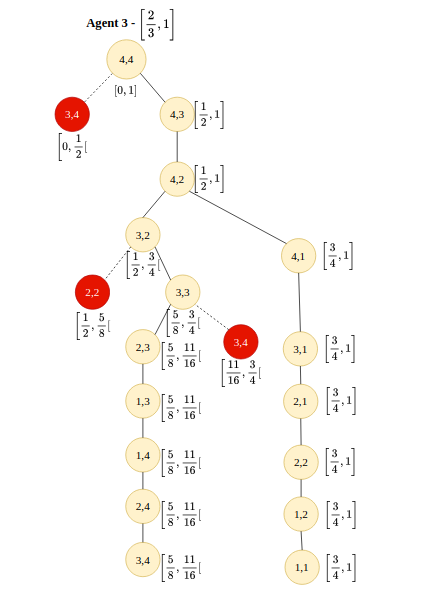
\includegraphics[width=1\textwidth]{ApeA/maze_agent_3_step_4.png}
    \caption{Agent 3 - Final exploration steps.}
    \label{fig_agent_3_step_4}
\end{figure}

